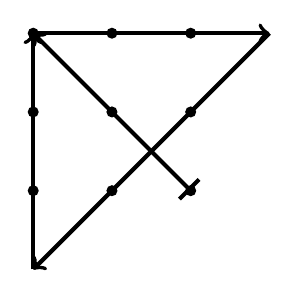
\begin{tikzpicture}[baseline=(current bounding box.north)]
    \fill (0,0) circle (2pt);
    \fill (0,1) circle (2pt);
    \fill (0,2) circle (2pt);

    \fill (1,0) circle (2pt);
    \fill (1,1) circle (2pt);
    \fill (1,2) circle (2pt);

    \fill (2,0) circle (2pt);
    \fill (2,1) circle (2pt);
    \fill (2,2) circle (2pt);

    %Linea que une los puntos
    \draw[line width=1.5,|->] (2,0) -- (0,2);
    \draw[line width=1.5,->] (0,2) -- (3,2);
    \draw[line width=1.5,->] (3,2) -- (0,-1);
    \draw[line width=1.5,->] (0,-1) -- (0,2);

\end{tikzpicture}

